\documentclass[12pt,a4paper]{article}
\usepackage[utf8]{inputenc}
\usepackage[usenames,dvipsnames]{xcolor}
\usepackage{tikz}
\usepackage{graphicx}
\usepackage{float}
\usepackage{subfig}
%\usepackage{subfigure}
\usepackage{multirow}
\usepackage{caption}
\usepackage{subcaption}
\usepackage{float}
\usepackage{listings}
\usepackage{natbib}
\usepackage{geometry}
\usepackage{array}
\usepackage[nottoc]{tocbibind}
\geometry{margin=2cm}
%set the indentation length to zero
\setlength{\parindent}{0pt}
\usepackage{hyperref}
\hypersetup{
    colorlinks=true,
    linkcolor=Black,
  filecolor=TUMBlue,      
    urlcolor=TUMBlue,
    citecolor=TUMBlue,
}



\urlstyle{same}
\graphicspath{ {./Figure/} }
\rmfamily
%set your name here
\newcommand*{\getAuthor}{Author}
%set your Submission Date here
\newcommand*{\getSubDate}{Submission date}
\newcommand*{\getSubLoc}{Munich}
\definecolor{TUMBlue}{cmyk}{1,0.43,0,0}
\newcommand\AtPageUpperRight[1]{\AtPageUpperLeft{%
   \makebox[\paperwidth][r]{#1}}}

\title{TUM-Document-Latex}

\author{llqqyyllqqyy }
\date{March 2020}

\begin{document}
\begin{titlepage}
\begin{tikzpicture}[remember picture,overlay]
   \node[anchor=north east,inner sep=20pt] at (current page.north east)
              {
\includegraphics[scale=0.06]{logo}};
\end{tikzpicture}
\vspace{50mm}

\centering
{\Huge\bfseries
Title
}

\vspace{130mm}
\large{
\begin{tabular}{l l}
    \bfseries{Author}:          & \getAuthor \\
    \bfseries{Supervisor}:      & Supervisor name \\
    \bfseries{Advisor}:         & Advisor\\
    \bfseries{Submission Date}: & Submission Date \\
  \end{tabular}
  }
\end{titlepage}

\cleardoublepage{}

\thispagestyle{empty}
\begin{center}{\Huge Declaration of Authorship}
\end{center}

\vspace*{0.1\textheight}
\noindent
\makeatletter
I hereby declare that the thesis submitted is my own unaided work. All direct or indirect sources used are acknowledged as references. I am aware that the thesis in digital form can be examined for the use of unauthorized
aid and in order to determine whether the thesis as a whole or parts incorporated
in it may be deemed as plagiarism. For the comparison of my work with existing
sources I agree that it shall be entered in a database where it shall also remain
after examination, to enable comparison with future theses submitted. Further rights
of reproduction and usage, however, are not granted here. This paper was not previously presented to another examination board and has not
been published.
\makeatother

\vspace{15mm}
\noindent 
\getSubLoc,
\getSubDate
\hspace{50mm}
\getAuthor
 \hspace{50mm} 

\cleardoublepage{}

\tableofcontents

\pagenumbering{Roman}%
%\tableofcontents%


\clearpage
\listoffigures
\clearpage
\listoftables{}
\clearpage
\addcontentsline{toc}{section}{Listings}
\lstlistoflistings
\clearpage
\addcontentsline{toc}{section}{Abstract}
\section*{Abstract}
\input{Abstract.tex}
\clearpage

\pagenumbering{arabic}%

\section{Introduction}
\subsection{Subsection}
\subsubsection{Subsubsection}
\paragraph{paragraph}
Cite here \cite{latex}


\section{Figure}
Following picture is Figure.\ref{Firework}

\begin{figure}[H]
\centering
\includegraphics[width=\linewidth,height=10cm,keepaspectratio]{Figure/Firework.JPG}
\caption{Firework}
\label{Firework}
\end{figure}


\begin{figure}[H]
\centering
\begin{minipage}{.5\linewidth}
  \centering
  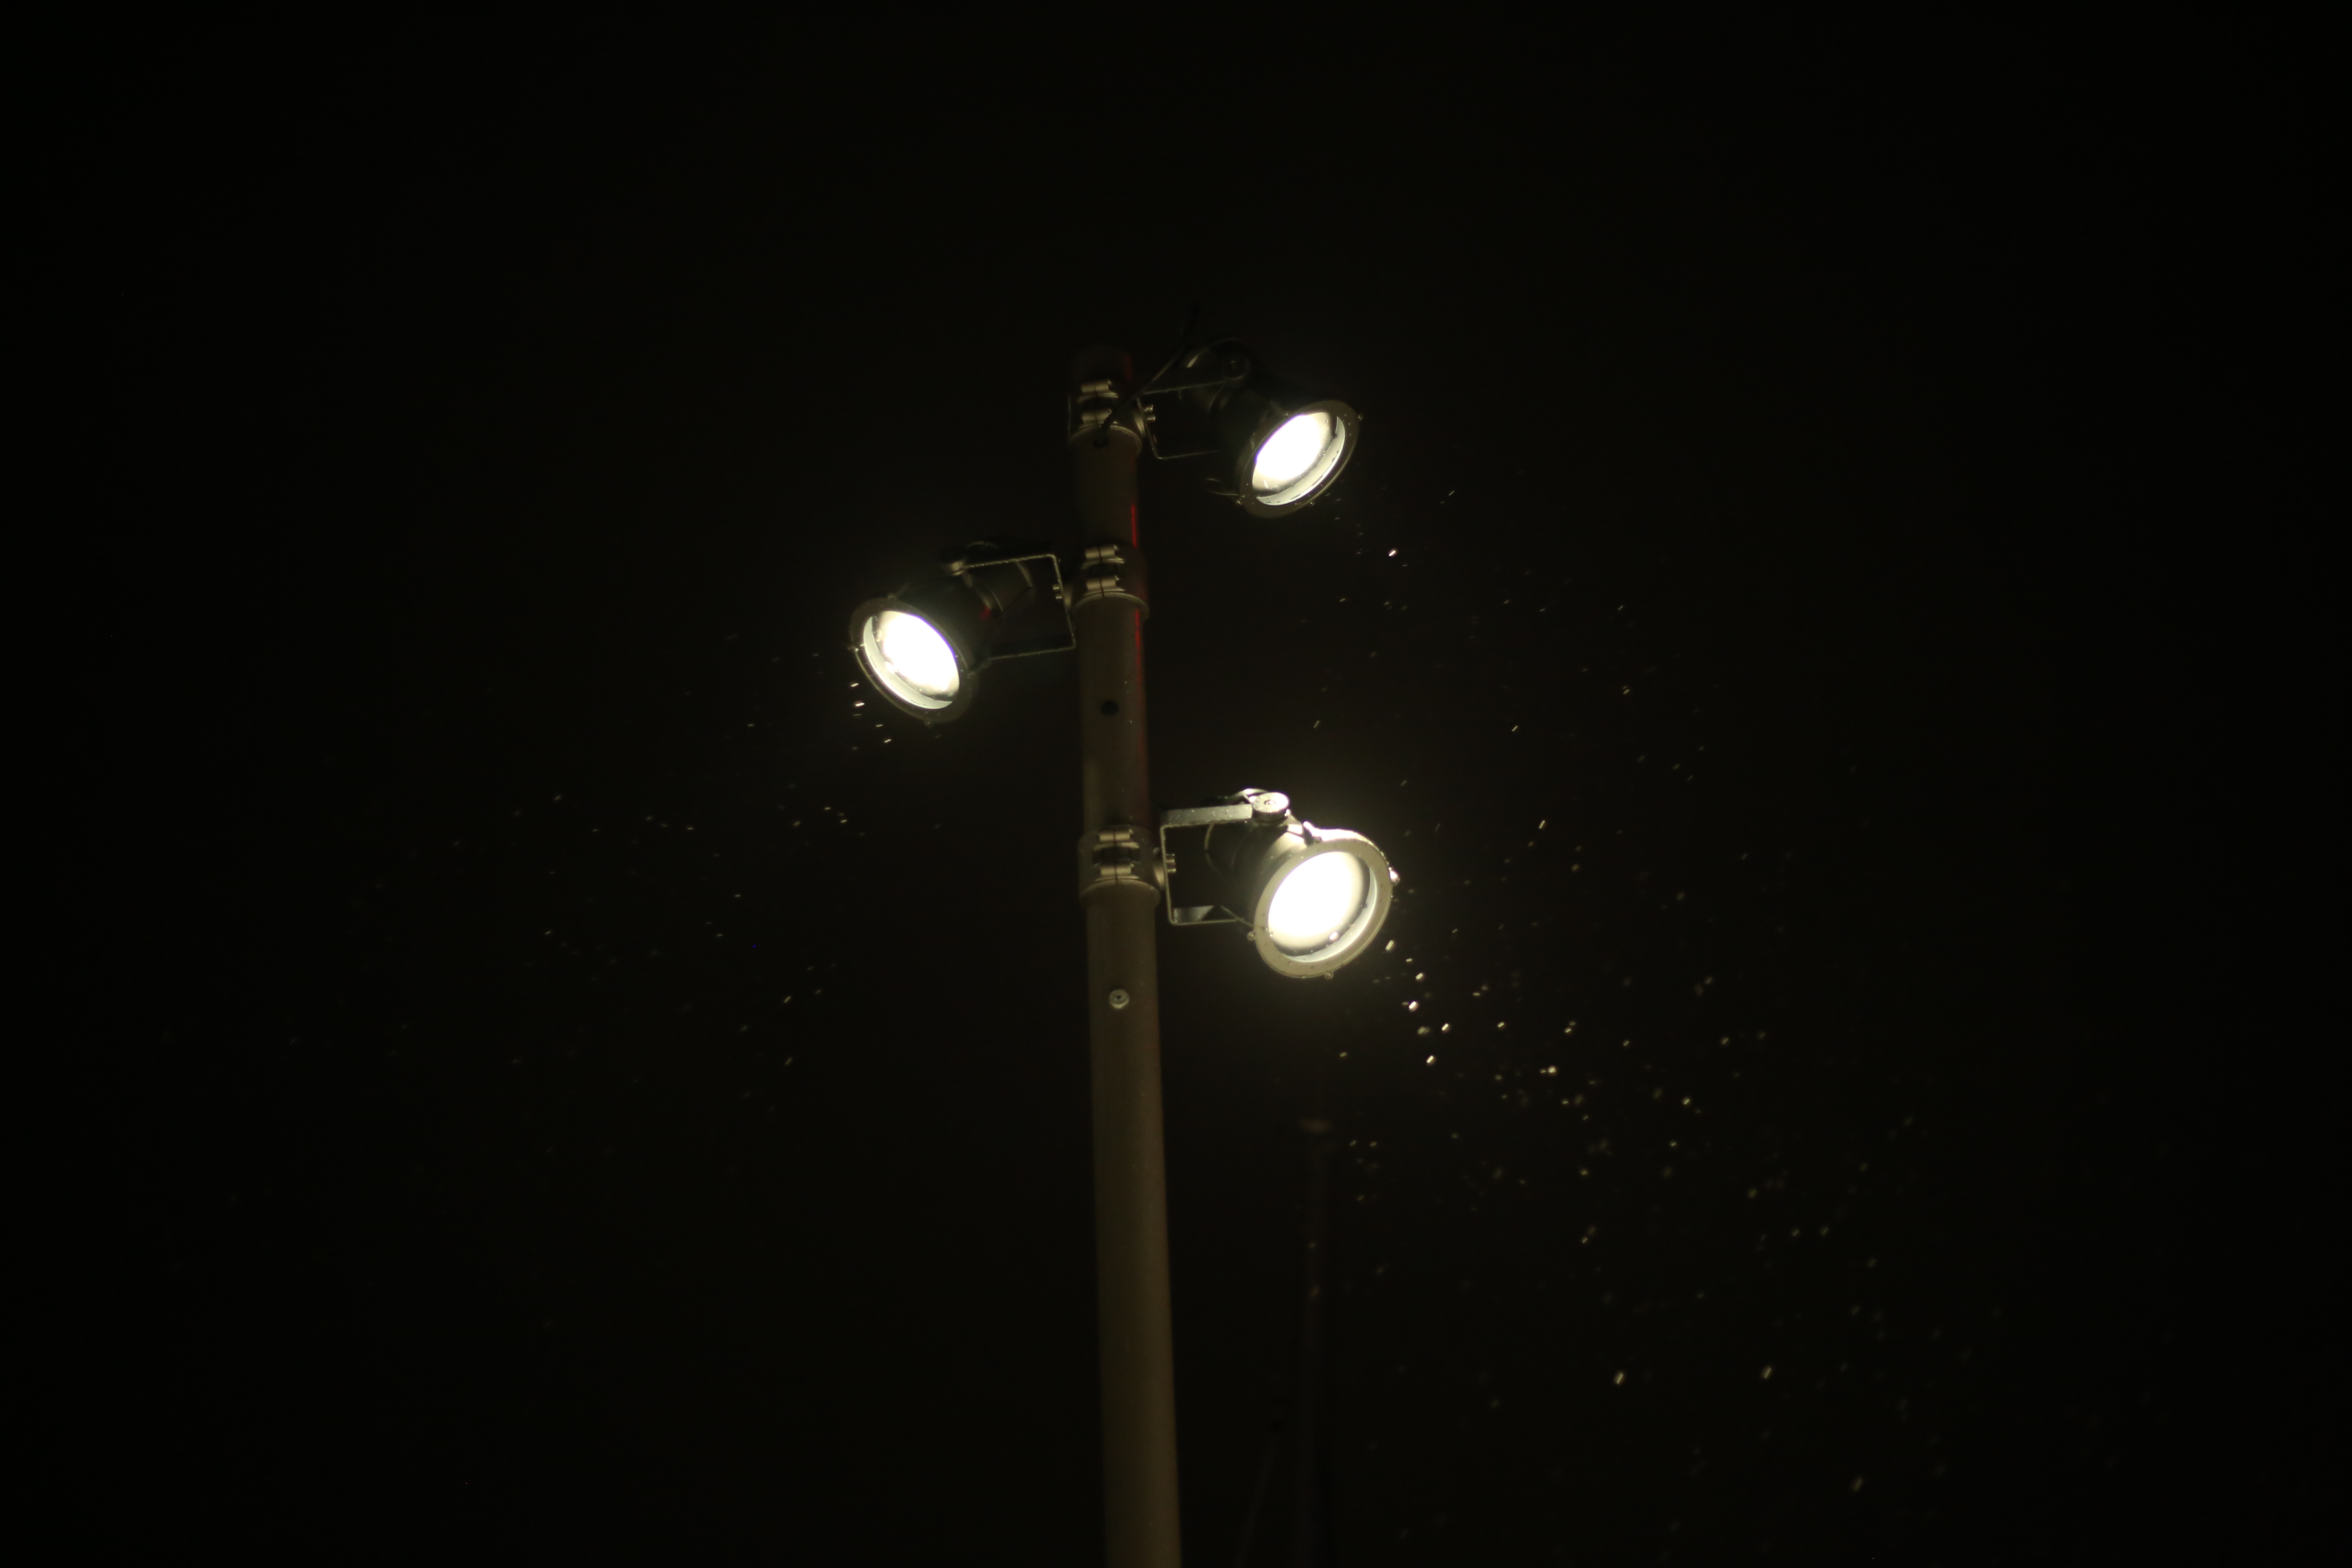
\includegraphics[width=.7\linewidth]{light}
  \captionof{figure}{A figure}
  \label{fig:test1}
\end{minipage}%
\begin{minipage}{.5\linewidth}
  \centering
  \includegraphics[width=.7\linewidth]{view}
  \captionof{figure}{Another figure}
  \label{fig:test2}
\end{minipage}
\end{figure}


\begin{figure*}[t]
\centering
\begin{tabular}{@{}ccc@{}}
\subfloat[a]{\includegraphics[width=0.3\textwidth]{Firework}} & 
\subfloat[b]{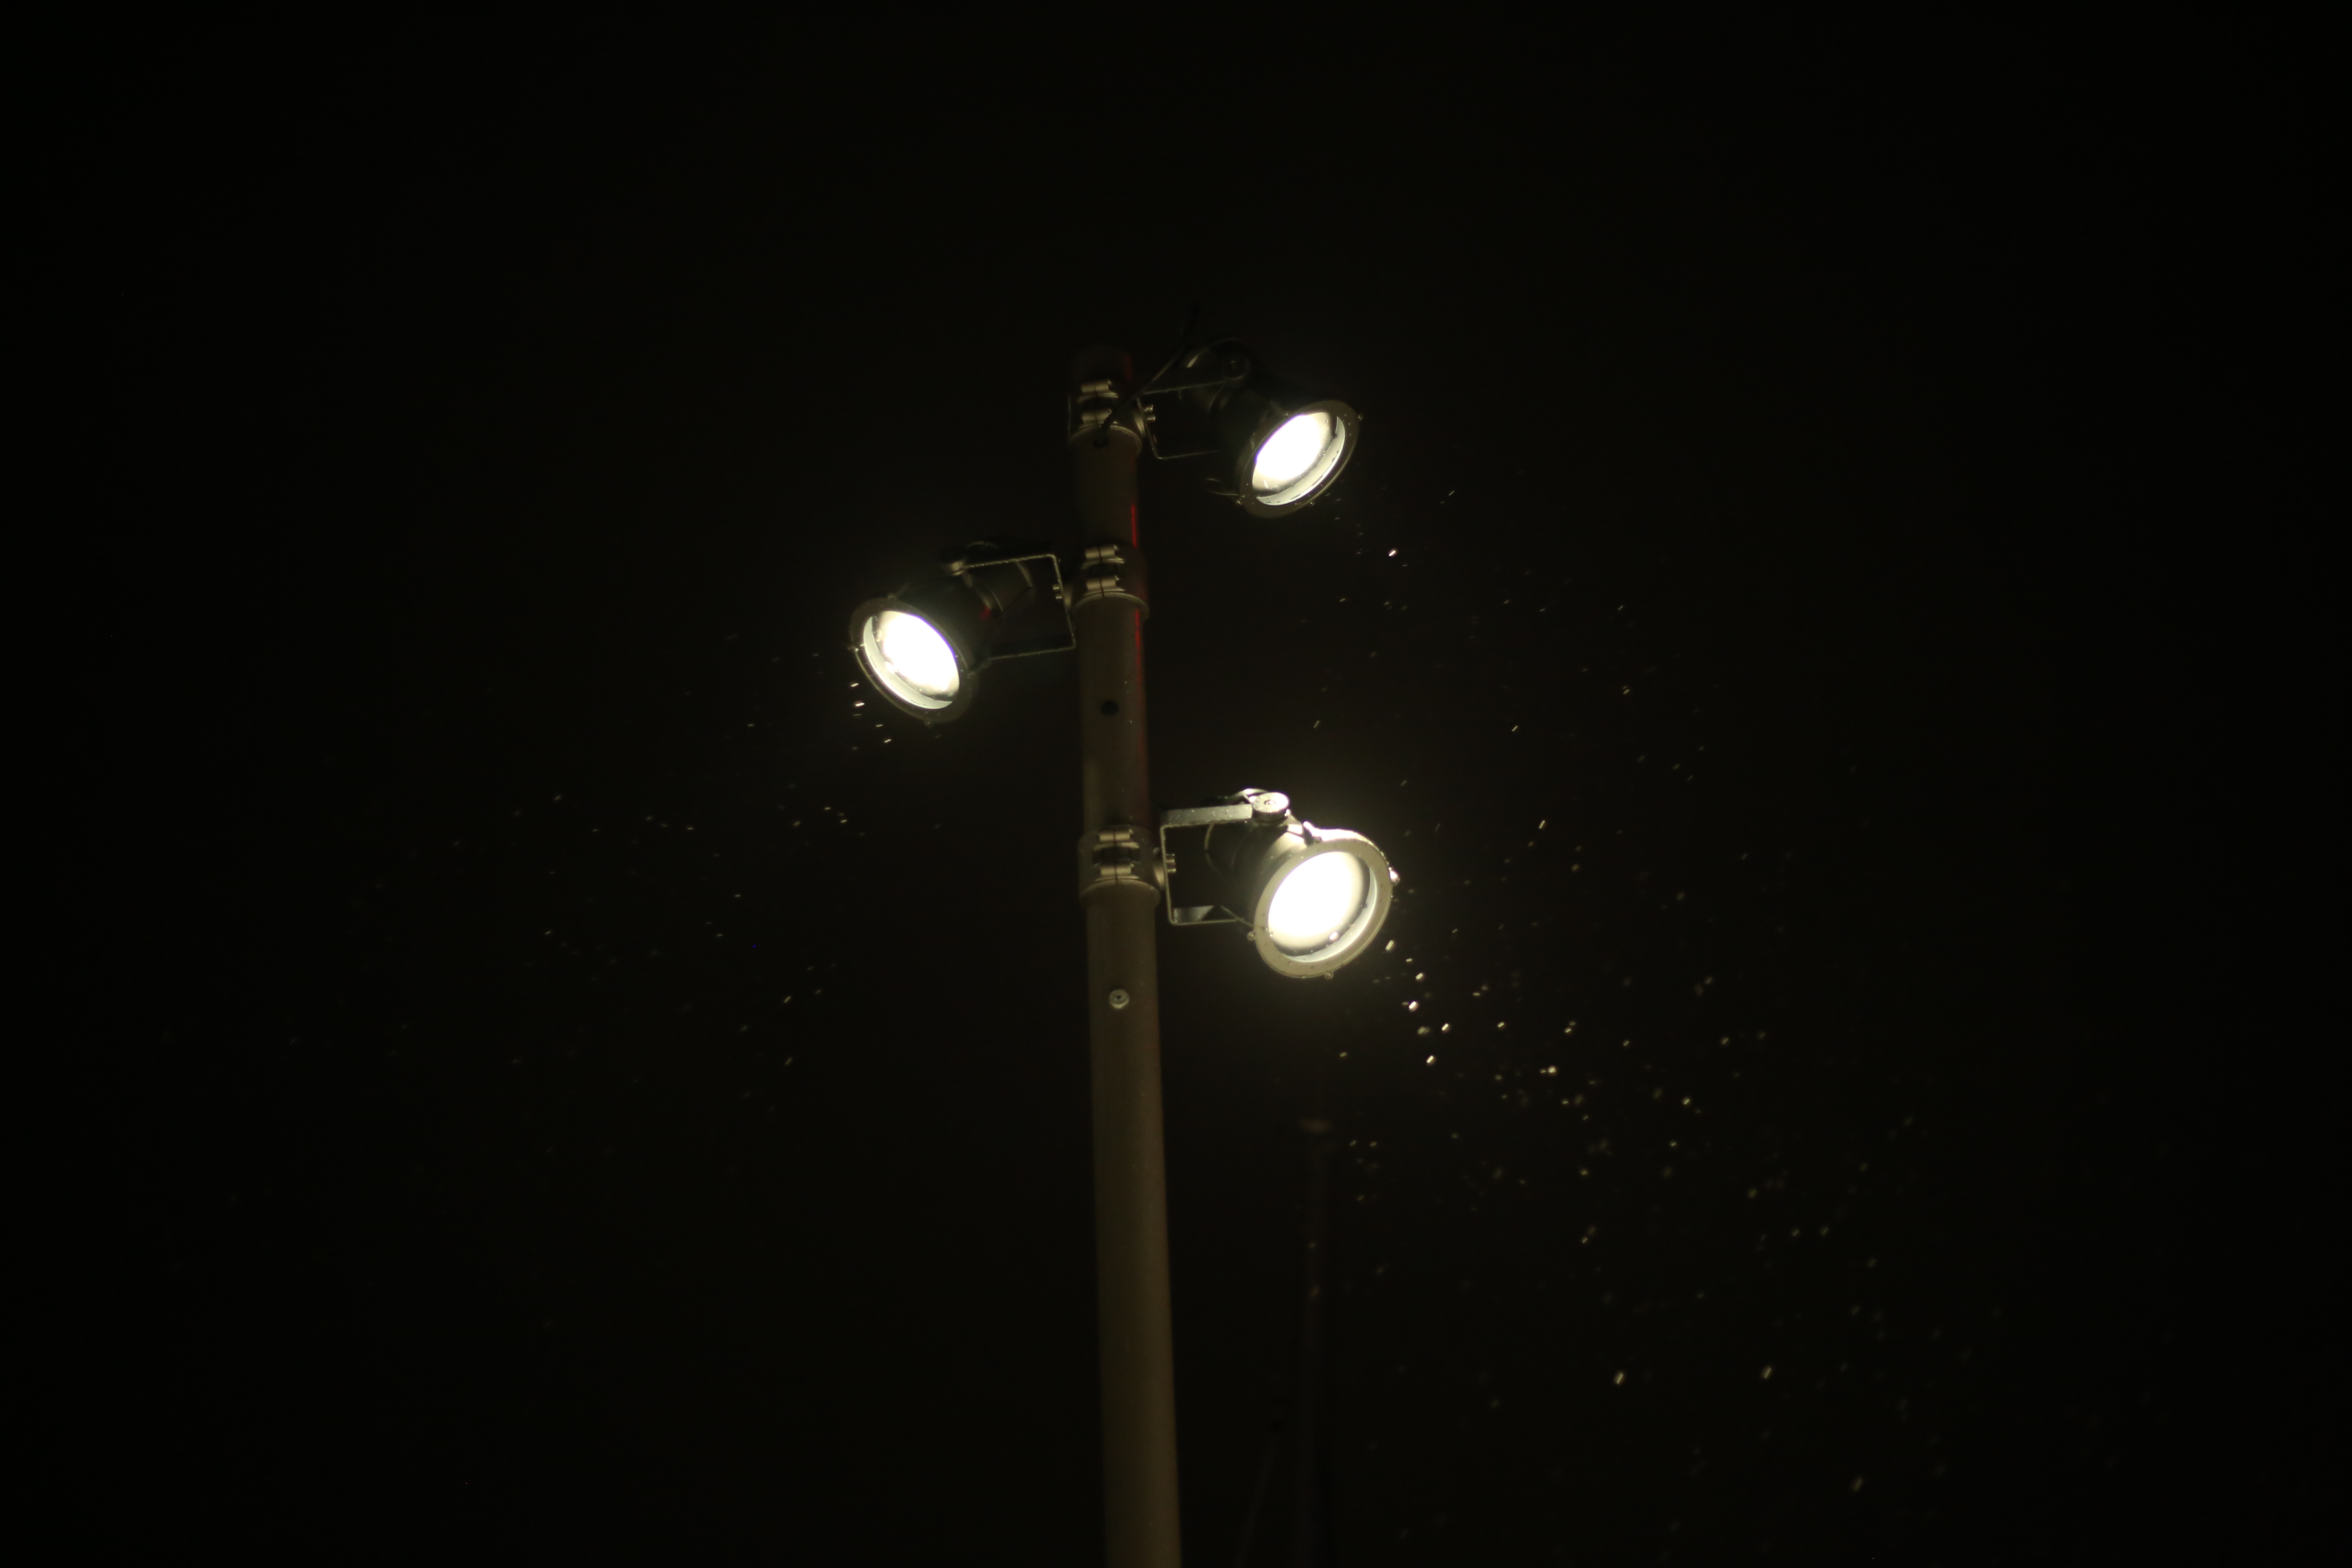
\includegraphics[width=0.3\textwidth]{light}} &
\subfloat[c]{\includegraphics[width=0.3\textwidth]{view}} \\
\end{tabular}
\caption[]{Description}
\label{fig:ABC}
\end{figure*}



\clearpage
\section{Table}
  \begin{tabular}{|m{0.2\textwidth}|m{0.2\textwidth}|m{0.5\textwidth}|}
  \hline
  Diagram & Name & Explanation \\
  \hline
  %\hline
\begin{minipage}{.2\textwidth}
      \includegraphics[width=\linewidth, height=\linewidth]{Firework}
    \end{minipage}
    
 & Firework & Firework in Norway \\
 
  \hline
\begin{minipage}{.2\textwidth}
      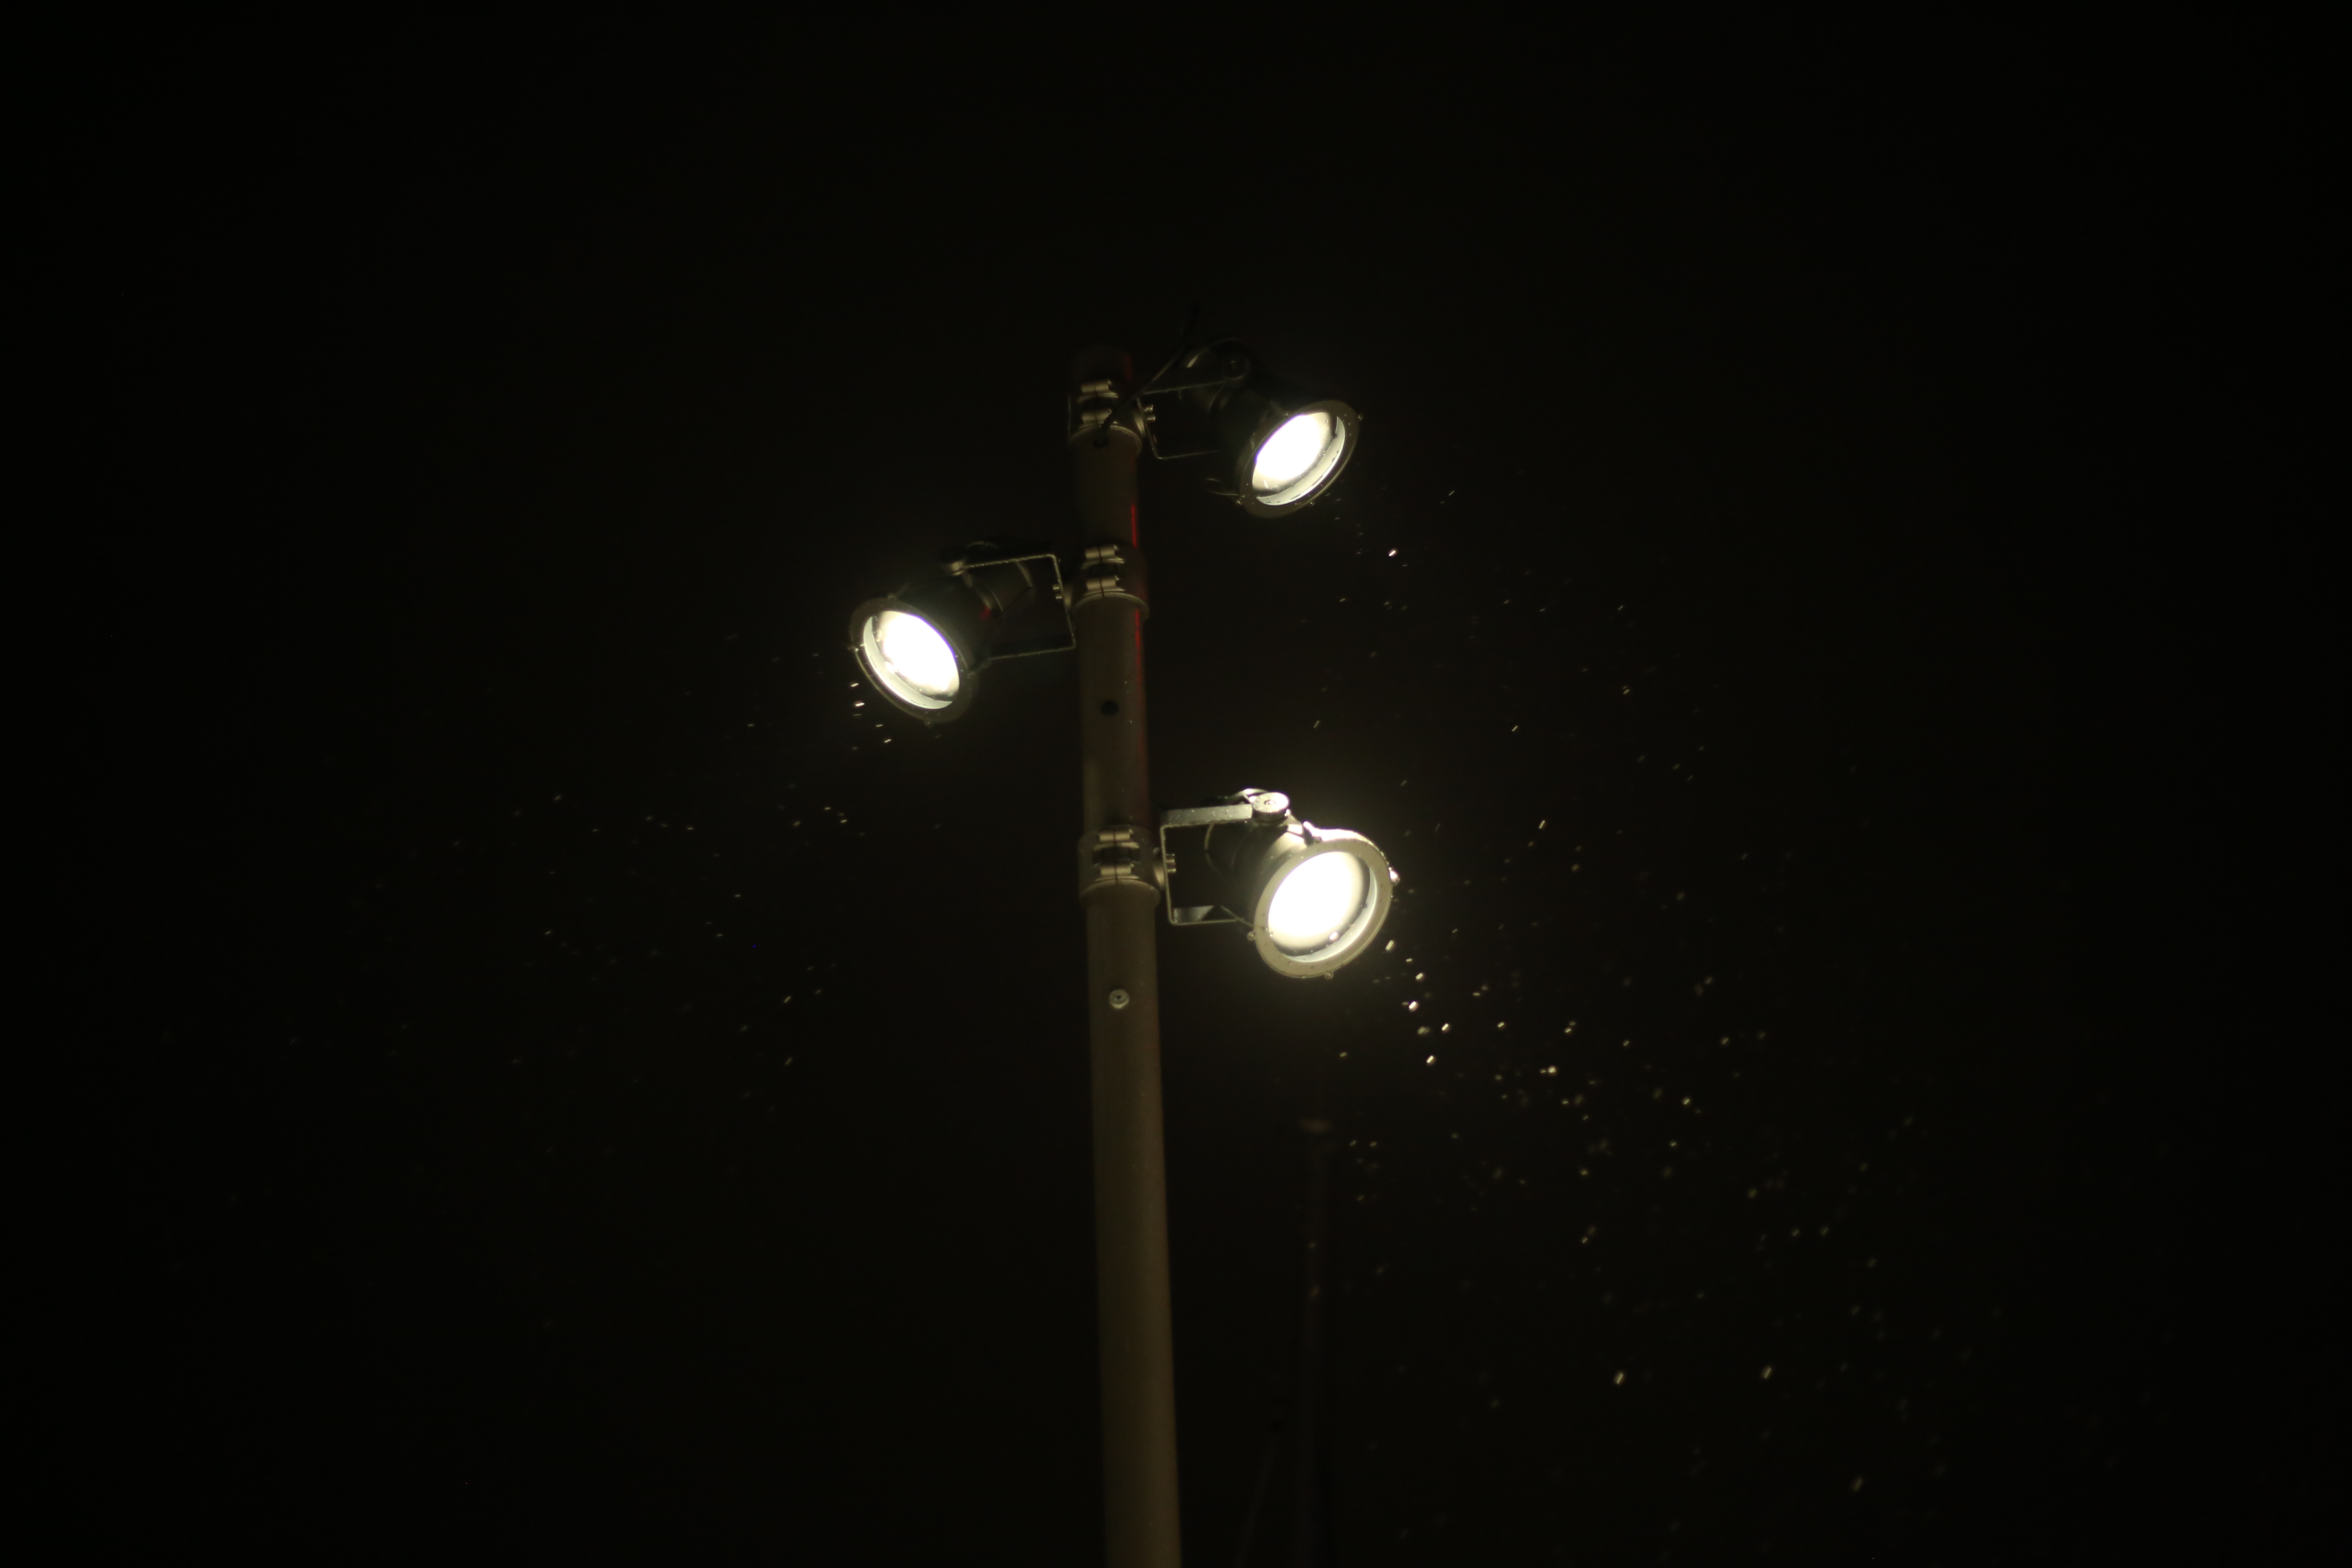
\includegraphics[width=\linewidth, height=\linewidth]{light}
    \end{minipage}
    
 & Light & Light in Norway \\

  \hline
     \begin{minipage}{.2\textwidth}
      \includegraphics[width=\linewidth, height=\linewidth]{view}
    \end{minipage}
    
 & View & View in Norway
 \\
  \hline
    
\end{tabular}

%list of code
\begin{lstlisting}[language=SQL, caption=SQL Script]
SELECT   "TABLE"."ID1" AS "ID"
FROM "SERVER"."TABLE" "TABLE"
Union All
SELECT   "TABLE"."ID2" AS "ID"
FROM "SERVER"."TABLE" "TABLE"

\end{lstlisting}
\clearpage

\section{Math}
Form 1:
\[ x^n + y^n = z^n \]

Form 2:
\begin{equation}
E=m
\end{equation}

Form 3:
$E=mc^2$

\vspace{8mm}
Others: check with the link: 
\url{https://www.overleaf.com/learn/latex/Subscripts_and_superscripts}

\clearpage
\renewcommand\bibname{References}
%APA Format Reference
\bibliographystyle{apalike}
\bibliography{reference.bib}
\addcontentsline{toc}{section}{Appendix}
\appendix
\end{document}
